%%%%%%%%%%%%%%%%%%%%%%%%%%%%%%%%%%%%%%%%%
%  My documentation report
%  Objetive: Explain what I did and how, so someone can continue with the investigation
%
% Important note:
% Chapter heading images should have a 2:1 width:height ratio,
% e.g. 920px width and 460px height.
%
%%%%%%%%%%%%%%%%%%%%%%%%%%%%%%%%%%%%%%%%%

%----------------------------------------------------------------------------------------
%	PACKAGES AND OTHER DOCUMENT CONFIGURATIONS
%----------------------------------------------------------------------------------------

\documentclass[11pt,fleqn]{book} % Default font size and left-justified equations

\usepackage[top=3cm,bottom=3cm,left=3.2cm,right=3.2cm,headsep=10pt,letterpaper]{geometry} % Page margins
\usepackage{pdfcolparallel}
\usepackage{listings}
\usepackage{xcolor} % Required for specifying colors by name
\definecolor{ocre}{RGB}{52,177,201} % Define the orange color used for highlighting throughout the book
\usepackage{graphicx}
\usepackage{subfig}
% Font Settings
\usepackage{avant} % Use the Avantgarde font for headings
%\usepackage{times} % Use the Times font for headings
\usepackage{mathptmx} % Use the Adobe Times Roman as the default text font together with math symbols from the Sym­bol, Chancery and Com­puter Modern fonts

\usepackage{microtype} % Slightly tweak font spacing for aesthetics
\usepackage[utf8]{inputenc} % Required for including letters with accents
\usepackage[T1]{fontenc} % Use 8-bit encoding that has 256 glyphs

% Bibliography
\usepackage[style=alphabetic,sorting=nyt,sortcites=true,autopunct=true,babel=hyphen,hyperref=true,abbreviate=false,backref=true,backend=biber]{biblatex}
\addbibresource{bibliography.bib} % BibTeX bibliography file
\defbibheading{bibempty}{}

%----------------------------------------------------------------------------------------
%	VARIOUS REQUIRED PACKAGES
%----------------------------------------------------------------------------------------

\usepackage{titlesec} % Allows customization of titles

\usepackage{graphicx} % Required for including pictures
\graphicspath{{Pictures/}} % Specifies the directory where pictures are stored

\usepackage{lipsum} % Inserts dummy text

\usepackage{tikz} % Required for drawing custom shapes

\usepackage[english]{babel} % English language/hyphenation

\usepackage{enumitem} % Customize lists
\setlist{nolistsep} % Reduce spacing between bullet points and numbered lists

\usepackage{booktabs} % Required for nicer horizontal rules in tables

\usepackage{eso-pic} % Required for specifying an image background in the title page

%----------------------------------------------------------------------------------------
%	MAIN TABLE OF CONTENTS
%----------------------------------------------------------------------------------------

\usepackage{titletoc} % Required for manipulating the table of contents

\contentsmargin{0cm} % Removes the default margin
% Chapter text styling
\titlecontents{chapter}[1.25cm] % Indentation
{\addvspace{15pt}\large\sffamily\bfseries} % Spacing and font options for chapters
{\color{ocre!60}\contentslabel[\Large\thecontentslabel]{1.25cm}\color{ocre}} % Chapter number
{}  
{\color{ocre!60}\normalsize\sffamily\bfseries\;\titlerule*[.5pc]{.}\;\thecontentspage} % Page number
% Section text styling
\titlecontents{section}[1.25cm] % Indentation
{\addvspace{5pt}\sffamily\bfseries} % Spacing and font options for sections
{\contentslabel[\thecontentslabel]{1.25cm}} % Section number
{}
{\sffamily\hfill\color{black}\thecontentspage} % Page number
[]
% Subsection text styling
\titlecontents{subsection}[1.25cm] % Indentation
{\addvspace{1pt}\sffamily\small} % Spacing and font options for subsections
{\contentslabel[\thecontentslabel]{1.25cm}} % Subsection number
{}
{\sffamily\;\titlerule*[.5pc]{.}\;\thecontentspage} % Page number
[] 

%----------------------------------------------------------------------------------------
%	MINI TABLE OF CONTENTS IN CHAPTER HEADS
%----------------------------------------------------------------------------------------

% Section text styling
\titlecontents{lsection}[0em] % Indendating
{\footnotesize\sffamily} % Font settings
{}
{}
{}

% Subsection text styling
\titlecontents{lsubsection}[.5em] % Indentation
{\normalfont\footnotesize\sffamily} % Font settings
{}
{}
{}
 
%----------------------------------------------------------------------------------------
%	PAGE HEADERS
%----------------------------------------------------------------------------------------

\usepackage{fancyhdr} % Required for header and footer configuration

\pagestyle{fancy}
\renewcommand{\chaptermark}[1]{\markboth{\sffamily\normalsize\bfseries\chaptername\ \thechapter.\ #1}{}} % Chapter text font settings
\renewcommand{\sectionmark}[1]{\markright{\sffamily\normalsize\thesection\hspace{5pt}#1}{}} % Section text font settings
\fancyhf{} \fancyhead[LE,RO]{\sffamily\normalsize\thepage} % Font setting for the page number in the header
\fancyhead[LO]{\rightmark} % Print the nearest section name on the left side of odd pages
\fancyhead[RE]{\leftmark} % Print the current chapter name on the right side of even pages
\renewcommand{\headrulewidth}{0.5pt} % Width of the rule under the header
\addtolength{\headheight}{2.5pt} % Increase the spacing around the header slightly
\renewcommand{\footrulewidth}{0pt} % Removes the rule in the footer
\fancypagestyle{plain}{\fancyhead{}\renewcommand{\headrulewidth}{0pt}} % Style for when a plain pagestyle is specified

% Removes the header from odd empty pages at the end of chapters
\makeatletter
\renewcommand{\cleardoublepage}{
\clearpage\ifodd\c@page\else
\hbox{}
\vspace*{\fill}
\thispagestyle{empty}
\newpage
\fi}

%----------------------------------------------------------------------------------------
%	THEOREM STYLES
%----------------------------------------------------------------------------------------

\usepackage{amsmath,amsfonts,amssymb,amsthm} % For math equations, theorems, symbols, etc

\newcommand{\intoo}[2]{\mathopen{]}#1\,;#2\mathclose{[}}
\newcommand{\ud}{\mathop{\mathrm{{}d}}\mathopen{}}
\newcommand{\intff}[2]{\mathopen{[}#1\,;#2\mathclose{]}}
\newtheorem{notation}{Notation}[chapter]

%%%%%%%%%%%%%%%%%%%%%%%%%%%%%%%%%%%%%%%%%%%%%%%%%%%%%%%%%%%%%%%%%%%%%%%%%%%
%%%%%%%%%%%%%%%%%%%% dedicated to boxed/framed environements %%%%%%%%%%%%%%
%%%%%%%%%%%%%%%%%%%%%%%%%%%%%%%%%%%%%%%%%%%%%%%%%%%%%%%%%%%%%%%%%%%%%%%%%%%
\newtheoremstyle{ocrenumbox}% % Theorem style name
{0pt}% Space above
{0pt}% Space below
{\normalfont}% % Body font
{}% Indent amount
{\small\bf\sffamily\color{ocre}}% % Theorem head font
{\;}% Punctuation after theorem head
{0.25em}% Space after theorem head
{\small\sffamily\color{ocre}\thmname{#1}\nobreakspace\thmnumber{\@ifnotempty{#1}{}\@upn{#2}}% Theorem text (e.g. Theorem 2.1)
\thmnote{\nobreakspace\the\thm@notefont\sffamily\bfseries\color{black}---\nobreakspace#3.}} % Optional theorem note
\renewcommand{\qedsymbol}{$\blacksquare$}% Optional qed square

\newtheoremstyle{blacknumex}% Theorem style name
{5pt}% Space above
{5pt}% Space below
{\normalfont}% Body font
{} % Indent amount
{\small\bf\sffamily}% Theorem head font
{\;}% Punctuation after theorem head
{0.25em}% Space after theorem head
{\small\sffamily{\tiny\ensuremath{\blacksquare}}\nobreakspace\thmname{#1}\nobreakspace\thmnumber{\@ifnotempty{#1}{}\@upn{#2}}% Theorem text (e.g. Theorem 2.1)
\thmnote{\nobreakspace\the\thm@notefont\sffamily\bfseries---\nobreakspace#3.}}% Optional theorem note

\newtheoremstyle{blacknumbox} % Theorem style name
{0pt}% Space above
{0pt}% Space below
{\normalfont}% Body font
{}% Indent amount
{\small\bf\sffamily}% Theorem head font
{\;}% Punctuation after theorem head
{0.25em}% Space after theorem head
{\small\sffamily\thmname{#1}\nobreakspace\thmnumber{\@ifnotempty{#1}{}\@upn{#2}}% Theorem text (e.g. Theorem 2.1)
\thmnote{\nobreakspace\the\thm@notefont\sffamily\bfseries---\nobreakspace#3.}}% Optional theorem note

%%%%%%%%%%%%%%%%%%%%%%%%%%%%%%%%%%%%%%%%%%%%%%%%%%%%%%%%%%%%%%%%%%%%%%%%%%%
%%%%%%%%%%%%% dedicated to non-boxed/non-framed environements %%%%%%%%%%%%%
%%%%%%%%%%%%%%%%%%%%%%%%%%%%%%%%%%%%%%%%%%%%%%%%%%%%%%%%%%%%%%%%%%%%%%%%%%%
\newtheoremstyle{ocrenum}% % Theorem style name
{5pt}% Space above
{5pt}% Space below
{\normalfont}% % Body font
{}% Indent amount
{\small\bf\sffamily\color{ocre}}% % Theorem head font
{\;}% Punctuation after theorem head
{0.25em}% Space after theorem head
{\small\sffamily\color{ocre}\thmname{#1}\nobreakspace\thmnumber{\@ifnotempty{#1}{}\@upn{#2}}% Theorem text (e.g. Theorem 2.1)
\thmnote{\nobreakspace\the\thm@notefont\sffamily\bfseries\color{black}---\nobreakspace#3.}} % Optional theorem note
\renewcommand{\qedsymbol}{$\blacksquare$}% Optional qed square
\makeatother

% Defines the theorem text style for each type of theorem to one of the three styles above
\newcounter{dummy} 
\numberwithin{dummy}{section}
\theoremstyle{ocrenumbox}
\newtheorem{theoremeT}[dummy]{Theorem}
\newtheorem{problem}{Problem}[chapter]
\newtheorem{exerciseT}{Exercise}[chapter]
\theoremstyle{blacknumex}
\newtheorem{exampleT}{Example}[chapter]
\theoremstyle{blacknumbox}
\newtheorem{vocabulary}{Vocabulary}[chapter]
\newtheorem{definitionT}{Definition}[section]
\newtheorem{corollaryT}[dummy]{Corollary}
\theoremstyle{ocrenum}
\newtheorem{proposition}[dummy]{Proposition}

%----------------------------------------------------------------------------------------
%	DEFINITION OF COLORED BOXES
%----------------------------------------------------------------------------------------

\RequirePackage[framemethod=default]{mdframed} % Required for creating the theorem, definition, exercise and corollary boxes

% Theorem box
\newmdenv[skipabove=7pt,
skipbelow=7pt,
backgroundcolor=black!5,
linecolor=ocre,
innerleftmargin=5pt,
innerrightmargin=5pt,
innertopmargin=5pt,
leftmargin=0cm,
rightmargin=0cm,
innerbottommargin=5pt]{tBox}

% Exercise box	  
\newmdenv[skipabove=7pt,
skipbelow=7pt,
rightline=false,
leftline=true,
topline=false,
bottomline=false,
backgroundcolor=ocre!10,
linecolor=ocre,
innerleftmargin=5pt,
innerrightmargin=5pt,
innertopmargin=5pt,
innerbottommargin=5pt,
leftmargin=0cm,
rightmargin=0cm,
linewidth=4pt]{eBox}	

% Definition box
\newmdenv[skipabove=7pt,
skipbelow=7pt,
rightline=false,
leftline=true,
topline=false,
bottomline=false,
linecolor=ocre,
innerleftmargin=5pt,
innerrightmargin=5pt,
innertopmargin=0pt,
leftmargin=0cm,
rightmargin=0cm,
linewidth=4pt,
innerbottommargin=0pt]{dBox}	

% Corollary box
\newmdenv[skipabove=7pt,
skipbelow=7pt,
rightline=false,
leftline=true,
topline=false,
bottomline=false,
linecolor=gray,
backgroundcolor=black!5,
innerleftmargin=5pt,
innerrightmargin=5pt,
innertopmargin=5pt,
leftmargin=0cm,
rightmargin=0cm,
linewidth=4pt,
innerbottommargin=5pt]{cBox}

% Creates an environment for each type of theorem and assigns it a theorem text style from the "Theorem Styles" section above and a colored box from above
\newenvironment{theorem}{\begin{tBox}\begin{theoremeT}}{\end{theoremeT}\end{tBox}}
\newenvironment{exercise}{\begin{eBox}\begin{exerciseT}}{\hfill{\color{ocre}\tiny\ensuremath{\blacksquare}}\end{exerciseT}\end{eBox}}				  
\newenvironment{definition}{\begin{dBox}\begin{definitionT}}{\end{definitionT}\end{dBox}}	
\newenvironment{example}{\begin{exampleT}}{\hfill{\tiny\ensuremath{\blacksquare}}\end{exampleT}}		
\newenvironment{corollary}{\begin{cBox}\begin{corollaryT}}{\end{corollaryT}\end{cBox}}	

%----------------------------------------------------------------------------------------
%	REMARK ENVIRONMENT
%----------------------------------------------------------------------------------------

\newenvironment{remark}{\par\vspace{10pt}\small % Vertical white space above the remark and smaller font size
\begin{list}{}{
\leftmargin=35pt % Indentation on the left
\rightmargin=25pt}\item\ignorespaces % Indentation on the right
\makebox[-2.5pt]{\begin{tikzpicture}[overlay]
\node[draw=ocre!60,line width=1pt,circle,fill=ocre!25,font=\sffamily\bfseries,inner sep=2pt,outer sep=0pt] at (-15pt,0pt){\textcolor{ocre}{R}};\end{tikzpicture}} % Orange R in a circle
\advance\baselineskip -1pt}{\end{list}\vskip5pt} % Tighter line spacing and white space after remark

%----------------------------------------------------------------------------------------
%	SECTION NUMBERING IN THE MARGIN
%----------------------------------------------------------------------------------------

\makeatletter
\renewcommand{\@seccntformat}[1]{\llap{\textcolor{ocre}{\csname the#1\endcsname}\hspace{1em}}}                    
\renewcommand{\section}{\@startsection{section}{1}{\z@}
{-4ex \@plus -1ex \@minus -.4ex}
{1ex \@plus.2ex }
{\normalfont\large\sffamily\bfseries}}
\renewcommand{\subsection}{\@startsection {subsection}{2}{\z@}
{-3ex \@plus -0.1ex \@minus -.4ex}
{0.5ex \@plus.2ex }
{\normalfont\sffamily\bfseries}}
\renewcommand{\subsubsection}{\@startsection {subsubsection}{3}{\z@}
{-2ex \@plus -0.1ex \@minus -.2ex}
{.2ex \@plus.2ex }
{\normalfont\small\sffamily\bfseries}}                        
\renewcommand\paragraph{\@startsection{paragraph}{4}{\z@}
{-2ex \@plus-.2ex \@minus .2ex}
{.1ex}
{\normalfont\small\sffamily\bfseries}}

%----------------------------------------------------------------------------------------
%	HYPERLINKS IN THE DOCUMENTS
%----------------------------------------------------------------------------------------

% For an unclear reason, the package should be loaded now and not later
\usepackage{hyperref}
\hypersetup{hidelinks,backref=true,pagebackref=true,hyperindex=true,colorlinks=false,breaklinks=true,urlcolor= ocre,bookmarks=true,bookmarksopen=false,pdftitle={Title},pdfauthor={Author}}

%----------------------------------------------------------------------------------------
%	CHAPTER HEADINGS
%----------------------------------------------------------------------------------------

% The set-up below should be (sadly) manually adapted to the overall margin page septup controlled by the geometry package loaded in the main.tex document. It is possible to implement below the dimensions used in the goemetry package (top,bottom,left,right)... TO BE DONE

\newcommand{\thechapterimage}{}
\newcommand{\chapterimage}[1]{\renewcommand{\thechapterimage}{#1}}

% Numbered chapters with mini tableofcontents
\def\thechapter{\arabic{chapter}}
\def\@makechapterhead#1{
\thispagestyle{empty}
{\centering \normalfont\sffamily
\ifnum \c@secnumdepth >\m@ne
\if@mainmatter
\startcontents
\begin{tikzpicture}[remember picture,overlay]
\node at (current page.north west)
{\begin{tikzpicture}[remember picture,overlay]
\node[anchor=north west,inner sep=0pt] at (0,0) {\includegraphics[width=\paperwidth]{\thechapterimage}};
%%%%%%%%%%%%%%%%%%%%%%%%%%%%%%%%%%%%%%%%%%%%%%%%%%%%%%%%%%%%%%%%%%%%%%%%%%%%%%%%%%%%%
% Commenting the 3 lines below removes the small contents box in the chapter heading
%\fill[color=ocre!10!white,opacity=.6] (1cm,0) rectangle (8cm,-7cm);
%\node[anchor=north west] at (1.1cm,.35cm) {\parbox[t][8cm][t]{6.5cm}{\huge\bfseries\flushleft \printcontents{l}{1}{\setcounter{tocdepth}{2}}}};
\draw[anchor=west] (5cm,-9cm) node [rounded corners=20pt,fill=ocre!10!white,text opacity=1,draw=ocre,draw opacity=1,line width=1.5pt,fill opacity=.6,inner sep=12pt]{\huge\sffamily\bfseries\textcolor{black}{\thechapter. #1\strut\makebox[22cm]{}}};
%%%%%%%%%%%%%%%%%%%%%%%%%%%%%%%%%%%%%%%%%%%%%%%%%%%%%%%%%%%%%%%%%%%%%%%%%%%%%%%%%%%%%
\end{tikzpicture}};
\end{tikzpicture}}
\par\vspace*{230\p@}
\fi
\fi}

% Unnumbered chapters without mini tableofcontents (could be added though) 
\def\@makeschapterhead#1{
\thispagestyle{empty}
{\centering \normalfont\sffamily
\ifnum \c@secnumdepth >\m@ne
\if@mainmatter
\begin{tikzpicture}[remember picture,overlay]
\node at (current page.north west)
{\begin{tikzpicture}[remember picture,overlay]
\node[anchor=north west,inner sep=0pt] at (0,0) {\includegraphics[width=\paperwidth]{\thechapterimage}};
\draw[anchor=west] (5cm,-9cm) node [rounded corners=20pt,fill=ocre!10!white,fill opacity=.6,inner sep=12pt,text opacity=1,draw=ocre,draw opacity=1,line width=1.5pt]{\huge\sffamily\bfseries\textcolor{black}{#1\strut\makebox[22cm]{}}};
\end{tikzpicture}};
\end{tikzpicture}}
\par\vspace*{230\p@}
\fi
\fi
}
\makeatother % Insert the commands.tex file which contains the majority of the structure behind the template

\definecolor{myviolet}{rgb}{0,0.6,0}
\definecolor{mygray}{rgb}{0.5,0.5,0.5}
\definecolor{mygreen}{rgb}{0,0.224,0.15}
\definecolor{myred}{rgb}{0.229,0,0}

\lstset{ %
  backgroundcolor=\color{white},   % choose the background color
  basicstyle=\footnotesize,        % size of fonts used for the code
  breaklines=true,                 % automatic line breaking only at whitespace
  captionpos=b,                    % sets the caption-position to bottom
  commentstyle=\color{myviolet},    % comment style
  escapeinside={\%*}{*)},          % if you want to add LaTeX within your code
  keywordstyle=\color{blue},       % keyword style
  stringstyle=\color{mygreen},
  numberstyle=\color{myred}     % string literal style
l}

\lstdefinestyle{BashStyle}{
  numbersep=10pt,
  tabsize=4,
  showspaces=false,
  showstringspaces=false
}

\begin{document}

%----------------------------------------------------------------------------------------
%	TITLE PAGE
%----------------------------------------------------------------------------------------

\begingroup
\thispagestyle{empty}
\AddToShipoutPicture*{\put(0,0){
\includegraphics[scale=1.00]{motherboard}}} % Image background
\centering
\vspace*{5cm}
\par\normalfont\fontsize{35}{35}\sffamily\selectfont
{\LARGE Università degli studi di Padova}\par % Book title
{\LARGE Corso di ingegneria dell'informazione}\par % Book title
{\LARGE Laboratorio di ingegneria informatica}\par % Book title
\vspace*{1.5cm}
\textbf{Link application}\\
\vspace*{1.5cm}
{\LARGE Anno accademico 2015-2016}\par % Book title

{\LARGE Davide Talon 1075692}\par % Author name
\endgroup

%----------------------------------------------------------------------------------------
%	COPYRIGHT PAGE
%----------------------------------------------------------------------------------------

\newpage
~\vfill
\thispagestyle{empty}

\noindent Copyright \copyright\ 2016 Davide Talon\\ % Copyright notice

\noindent \textsc{Laboratorio di ingegneria informatica, Università degli studi di Padova, Italia.}\\

\noindent \textsc{https://bitbucket.org/davidetalon/link}\\ % URL
\noindent \textsc{https://github.com/davidetalon/link}\\ % URL

\noindent Progetto per il laboratorio di ingegneria informatica, corso tenuto dal professore Nicola Ferro. Svolto nel secondo semestre dell'anno accademico 2015 - 2016.\\ % License information

%\noindent \textit{First release, August 2014} % Printing/edition date

%----------------------------------------------------------------------------------------
%	TABLE OF CONTENTS
%----------------------------------------------------------------------------------------

\chapterimage{airdrop} % Table of contents heading image

\pagestyle{empty} % No headers

\tableofcontents % Print the table of contents itself

%\cleardoublepage % Forces the first chapter to start on an odd page so it's on the right

\pagestyle{fancy} % Print headers again

%----------------------------------------------------------------------------------------
%	CHAPTER 1
%----------------------------------------------------------------------------------------

\chapterimage{earth} % Chapter heading image

\chapter{Introduzione}

\section{Contesto}\index{Contesto}

Seguendo il corso Laboratorio di ingegneria informatica il cui obiettivo è l'acquisizione di competenze di programmazione nel linguaggio C per applicarle a casi di interesse industriale ci è stato assegnato il seguente compito:

\begin{quote}
Realizzazione di un progetto individuale su un argomento di proprio interesse.
\end{quote}

\noindent Pertanto, pensando ai possibili sviluppi, mi sono imbattuto in un problema pratico.
Quante volte ci è capitato, in casa o in ufficio, di dover scambiare dei file tra computer vicini e di utilizzare le classiche introvabili chiavette o l'email il cui upload è lentissimo?
Nonostante l'avanzare della tecnologia, infatti, non disponiamo ancora di un metodo semplice e veloce per lo scambio di file tra computer vicini e, in particolare, per computer connessi alla stessa rete.
Gli utenti Apple già conoscono l'utilità di Airdrop che consente di inviare documenti, immagini e video ai computer vicini creando una rete ad hoc, ma perchè non estendere questa funzionalità a Linux, comprendendo dunque tutti i sistemi operativi Unix-like?
Nasce, dunque, la necessità di avere una applicazione multi-piattaforma che permette, in modo facile e veloce, di inviare file da un computer a un altro.



\section{Motivazioni}\index{Motivazioni}

Con l'occasione del Laboratorio di ingegneria informatica e la possibilità di sviluppare un progetto inerente ai propri interessi nasce l'applicazione Link che permette, a due computer connessi alla stessa rete, di scambiarsi dei file.
Questo progetto, infatti, parte principalmente dalla propria passione per internet e le telecomunicazioni, un mondo che mi appassiona e entusiasma facendomi capire la potenza delle nuove tecnologie.
Tante volte mi è capitato di dover inviare dei file da un computer ad un altro e mi sono sempre chiesto quale fosse un metodo pratico e veloce per farlo, quindi ciò che ha spinto allo sviluppo di questo progetto è la ricerca di una soluzione personale per risolvere un problema che si incontra spesso nella vita quotidiana.
Da qui l'idea di utilizzare la connessione locale per lo scambio di file.

\section{Obiettivi}\index{Obiettivi}


L'obiettivo primario del progetto è quello di sviluppare un'applicazione per inviare qualsiasi tipo di file tra computer connessi alla stessa rete e far in modo che tale applicazione sia disponibile per tutti i sistemi operativi Unix-like.
Le caratteristiche principali che il prodotto finale dovrà avere saranno intuitività nell'utilizzo, velocità di trasmissione e leggerezza:
\medskip
\begin{description}
\item[Intuitività]: l'applicazione sviluppata dovrà essere estremamente intuitiva e di facile comprensione, pertanto ci limitiamo a pochi comandi essenziali autoesplicativi.
\item [Velocità]: l'invio dei file deve avvenire in pochi semplici passaggi e potrà sfruttare la potenza della connessione locale.
\item [Leggerezza]: il programma sarà estremamente leggero e permetterà di inviare file di dimensioni arbitrariamente grandi senza doverli completamente caricare nella RAM, non influenzando le prestazioni generali del sistema durante l'esecuzione.
\end{description}

\medskip
\noindent Inoltre, seguendo la propria passione per le telecomunicazioni, tra gli obiettivi di questo progetto vi è quello di crescere nella conoscenza delle reti e dei socket oltre che nell'intero mondo Unix.
Volendo schematizzare gli obiettivi prefissati, si ha:
\medskip
\begin{itemize}
\item Permettere a un utente di inviare files da un computer a un altro.
\item Creare una applicazione multi-piattaforma disponibile per i SO Unix-like.
\item Semplicità e intuitività nell'utilizzo dell'applicazione.
\item Acquisire conoscenze di programmazione in C
\item Crescita personale nella conoscenza delle reti e del loro funzionamento.
\end{itemize}

\section{Link utili e installazione}\index{Link utili e installazione}
L'intero progetto, comprensivo di report finale e slides di presentazione è disponibile sia su Bitbucket \url https://bitbucket.org/davidetalon/link sia su GitHub alla pagina \url https://github.com/davidetalon/link da cui si possono scaricare i file sorgenti e quanto necessario per l'intallazione dell'applicazione.\\
\noindent In particolare per l'intallazione dell'applicazione:

\begin{enumerate}
	\item Crea la cartella dove installare link e spostati al suo interno
\begin{verbatim}
$ mkdir link
$ cd link
\end{verbatim}
    \item Scarica la repository da GitHub
\begin{verbatim}
$ git clone https://github.com/davidetalon/link.git
\end{verbatim}
    \item Compila tramite Cmake (è richiesta almeno la versione 3.4)
\begin{verbatim}
$ cmake .
$ make
\end{verbatim}
     \item Ti suggerisco di aggiungere link al path di sistema
\begin{verbatim}
$ PATH=<path to link>:$PATH
\end{verbatim}
	\item Ora puoi conoscere link utilizzando il suo help
\begin{verbatim}
$ link --help
\end{verbatim}
             
\end{enumerate}

\subsection{Licenza}\index{Licenza}

Tutto il codice è disponibile sotto la licenza Apache 2.0 "AS IS" BASIS, WITHOUT WARRANTIES OR CONDITIONS OF ANY KIND pertanto puoi sentirti libero di modificarlo e ridistribuirlo.
Puoi ottenere una copia della licenza al link 

    \url http://www.apache.org/licenses/LICENSE-2.0




%----------------------------------------------------------------------------------------
%	CHAPTER 2
%----------------------------------------------------------------------------------------
\chapterimage{softwaredesign.jpg}

\chapter{Progettazione}

\section{Idea iniziale}\index{Idea iniziale}

Deciso di sviluppare un software per lo scambio di file tra computer connessi alla stessa rete, si è passati alla fase di progettazione dell'applicazione Link.
L'idea di fondo è quella di creare un unico software che funzioni sia per la ricezione che per l'invio di dati, pertanto il software dovrà essere in grado di agire sia come server, ovvero in attesa di ricevere delle richieste, sia come client che richiede la connessione.
L'invio di un file deve avvenire in pochi semplici passaggi; Link permette di cercare tutti i dispositivi che sono in ascolto nella rete locale e lascia all'utente la scelta del destinatario.
Dunque, scelto il ricevente, l'applicazione si occuperà, tramite le varie chiamate di sistema, di comprimere i dati e di eseguire tutti i controlli necessari per la trasmissione dei dati.



\section{Architettura}\index{Architettura software}

Come già sottilineato la piattaforma deve essere in grado sia di interpretare il ruolo di server per poter ricevere i dati in ingresso, sia il ruolo di client per poter inviare i dati. Pertanto, per comprendere meglio il funzionamento dell'applicazione sono state definite due modalità operative:
\medskip
\begin{description}
\item[Master mode] : è la condizione di ricezione e attesa, infatti, la piattaforma si mette in ascolto su una specifica porta UDP e aspetta di ricevere una richiesta da parte di qualche mittente, ricevuta la richiesta, apre un socket TCP e legge i dati in ingresso.
\item [Sleave mode]: è la modalità con cui è possibile inviare un file, infatti, entrati in modalità sleave si cercano tutti i master in ascolto all'interno della rete e si trasmettono i dati.
\end{description}

\medskip
\noindent Volendo rendere l'applicazione disponibile per i sistemi operativi Unix-like la gestione delle connessioni è ricaduta sui \texttt{socket} di C offerti dalle API di Unix i quali hanno permesso di gestirle in modo piuttosto efficiente e di avere abbastanza libertà di decisione.\\
\noindent Il problema principale nella progettazione dell'architettura software è stata la non conoscenza della rete, infatti, generalmente, un server possiede un Ip statico, ma cosa succede con l'utilizzo del moderno DHCP in cui viene assegnato, all'interno della rete, un Ip casuale? E se la rete cambia?\\
\noindent Pertanto si è pensato a un modo per interrogare tutti i master disponibili sulla rete inviando un messaggio broadcast.\\
\noindent Per quanto riguarda la compressione, invece, si è scelto, per inter-compatibilità dei vari sistemi operativi di utilizzare \texttt{tar} disponibile, in varie versioni, su tutto il mondo Unix.\\
\noindent Analizziamo, nel dettaglio il funzionamento della piattaforma nelle prossime sezioni.

\subsection{Socket}
Per comprendere a fondo come è stata progettata l'applicazione è necessario, innanzitutto, comprendere cosa sono i Socket e il loro funzionamento.
I socket fanno parte della IPC (interprocess communication facilities) di Unix e permettono lo scambio di dati, oltre che sulla stessa macchina, anche tra più host connessi alla rete. Supponiamo di trovarci davanti alla classica architettura Client/Server:
\medskip

\begin{itemize}
	\item Ogni applicazione, sia lato server, che lato client, apre un socket ovvero una interfaccia che permette alle due applicazioni di comunicare l'una con l'altra
	\item Il server binda il socket su indirizzo conosciuto in modo che il client possa connettersi a lui
\end{itemize}
\medskip
Pertanto una trasmissione dati, a livello software, è caratterizzata da una coppia di socket che identificano rispettivamente il client e server
Nella piattaforma Link saranno necessari principalmente due tipo di Socket:
\medskip
\begin{itemize}
	\item  \texttt{SOCK\_STREAM} i socket di tipo stream ci permettono un canale di comunicazione affidabile, orientato alla connessione e byte-stream, ovvero:
	\begin{description}
		\item [Affidabile] viene garantito che i dati arrivino intatti al destinatario, ovvero così come sono stati trasmessi
		\item [Orientato alla connessione] viene garantito che i vari messaggi arrivo al destinatario nello stesso ordine in cui sono stati inviati
		\item [Byte-stram] non vi sono limiti di dimensioni alla quantità di dati che possono essere inviati
	\end{description}
	\obeylines
	\item	\texttt{SOCK\_DGRAM} i socket di tipo datagram ci permettono di inviare dati in modo più veloce, senza però assicurarci che la trasmissione dei dati sia corretta, essi infatti possono arrivare sbagliati al destinatario, non arrivare o arrivare in ordine diverso da quello di partenza
\end{itemize}
\medskip
\noindent In particolare verranno utilizzati i socket di tipo \texttt{AF\_INET} che permette lo scambio di dati tra host connessi in rete tramite il protocolo \textit{Ipv4}.

\noindent Per bindare il socket del server, ovvero assegnargli un indirizzo noto dovremmo assegnargli una precisa porta in cui ascoltare, mentre per quanto riguarda l'indirizzo Ip, possiamo assegnargli tranquillamente \texttt{INADDR\_ANY} ovvero l'interfaccia di loopback che permette di indirizzare il socket su tutte le interfacce di rete disponibili.

\begin{remark}
	Uteriori informazioni sui socket e il loro funzionamento, insieme ad innumerevoli esempi possono essere trovati alla pagina \url http://http://www.beej.us/guide/bgnet/ e su \textit{The linux programming interface: A Linux and UNIX System Programming Handbook, M. Kerrisk, Nostark, 2010.}

\end{remark}

\begin{figure}[h]
    \centering
    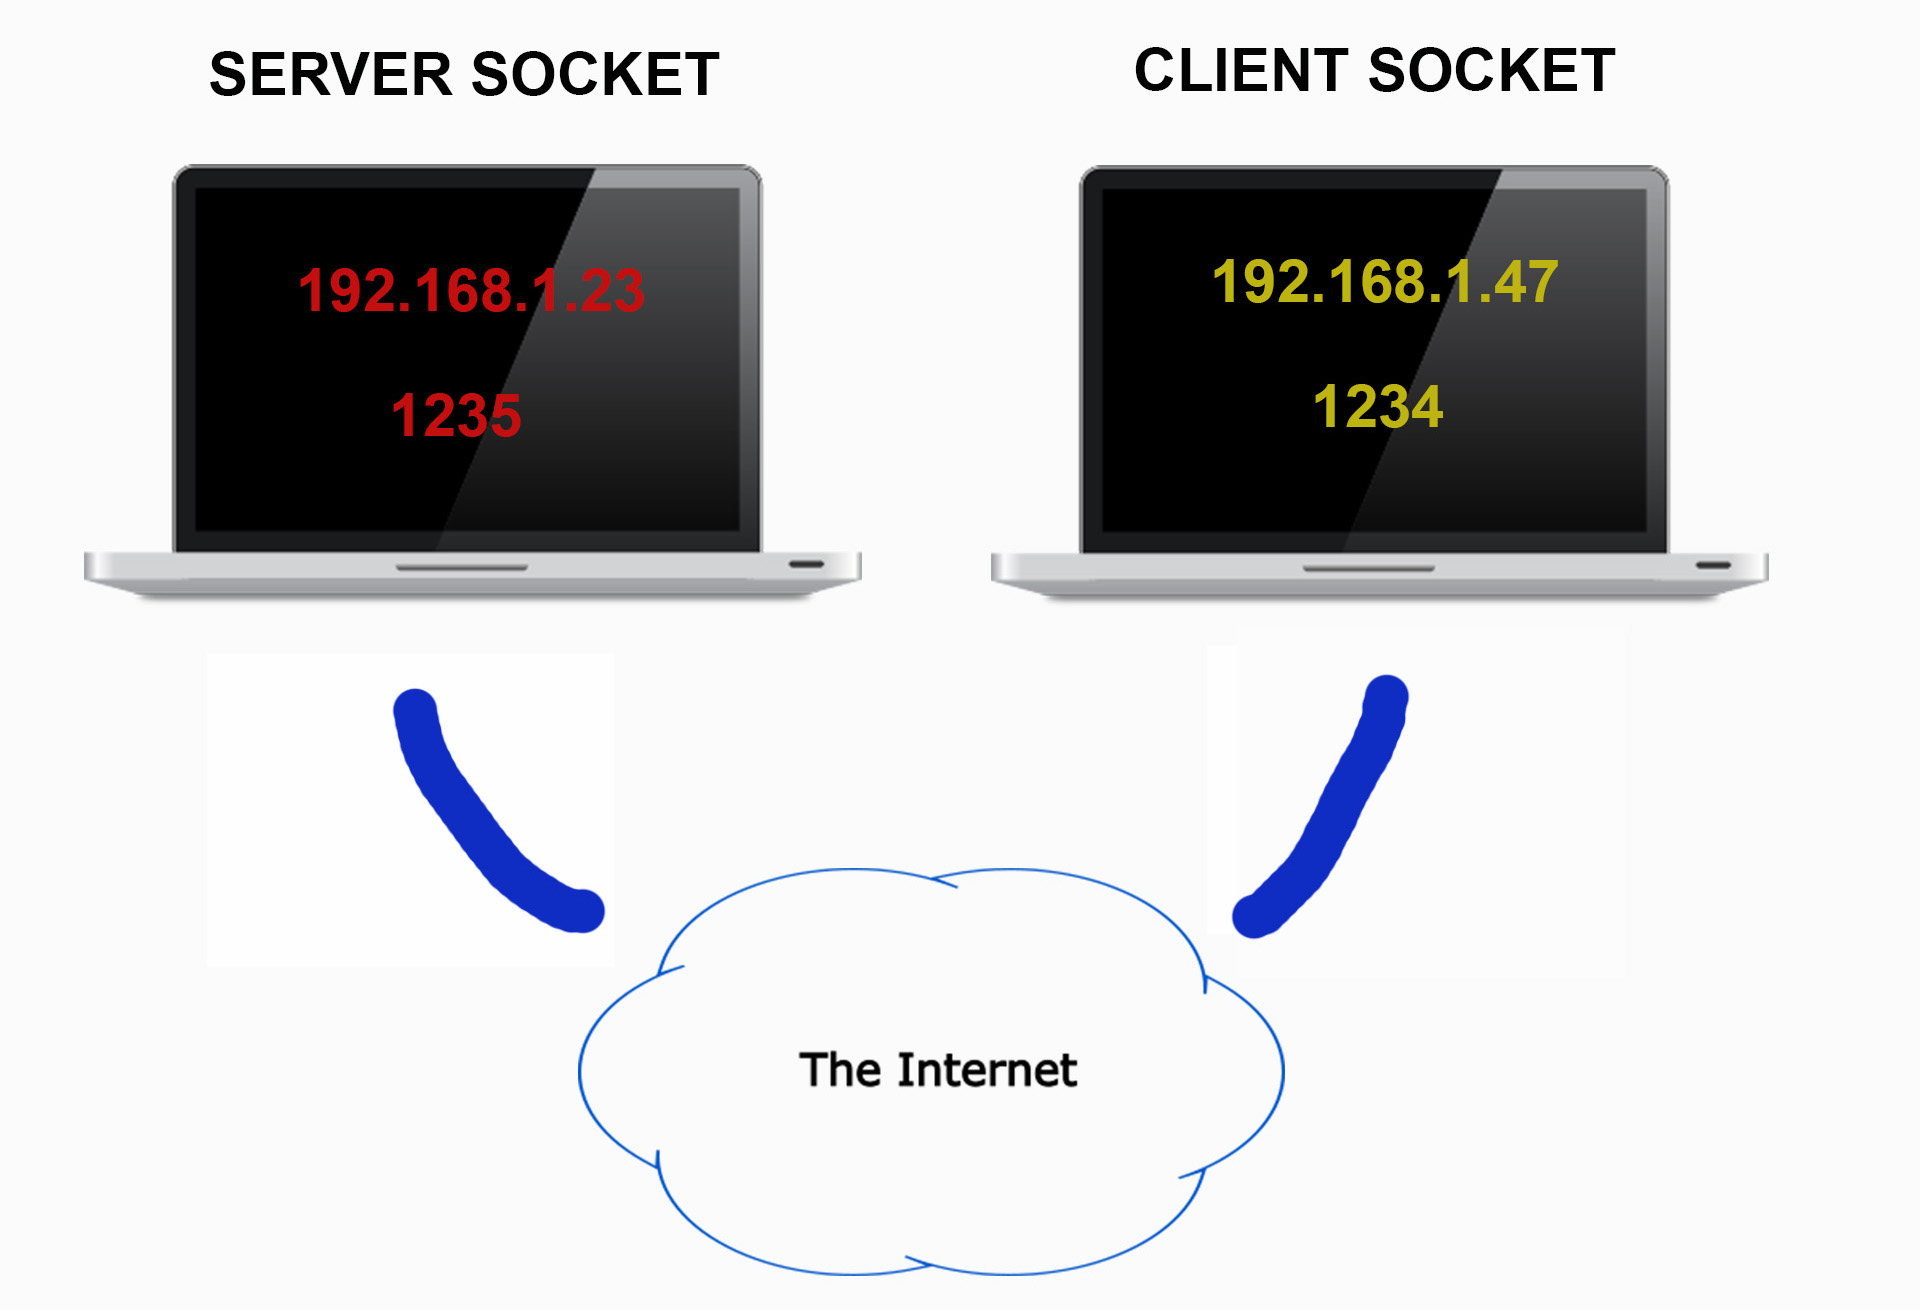
\includegraphics[width=0.77\textwidth]{socket.jpg}
    \caption{Principio di funzionamento dei socket, la trasmissione è identificata da una copia di socket.}
    \label{fig:awesome_image}
\end{figure}


\subsection{Sleave}
Come già anticipato, nella modalità sleave è possibile inviare i file al destinatario scelto, per far questo entrati nella sleave mode la piattaforma apre un socket UDP sulla porta 1234 e invia un messaggio in broadcast sulla porta 1235 interrogando tutti i Link master in ascolto sulla rete locale.
Viene, infatti, inviata la richiesta \texttt{LINKAPP/CLNTRQT/SRVON?/} e si mette in ascolto delle eventuali risposte da parte dei master disponibili.
Verificata la correttezza della risposta, dunque, tutti i master validi vengono messi in un array contenente il loro nome e l'indirizzo del loro socket.
A questo punto l'applicazione, elencando i vari master disponibili nella rete, permette, in modo interattivo, di scegliere il destinatario e di inviare i file.
La piattaforma si preoccupa, quindi, di preparare il file da trasmettere comprimendolo come specificato nei prossimi paragrafi.
In particolar modo, conoscendo l'indirizzo del ricevente, lo sleave apre un socket TCP sulla porta 2345, effettua una richiesta di connessione al master scelto e, inviando nei primi byte trasmessi il messaggio \texttt{LINKAPP/SLVNAME/<nomesleave>/FNAME/<nomefiledainviare>}, chiede se accetta di ricevere il file.
Vengono dunque raccolte informazioni sul file da trasmettere e in particolare la dimensione del file, la quale viene inviata al master connesso.
Il file viene dunque aperto in lettura e inviato allo sleave senza caricarlo interamente in memoria centrale ma limitandosi a un buffer di 4 MB.

\begin{figure}[h]
	\centering
    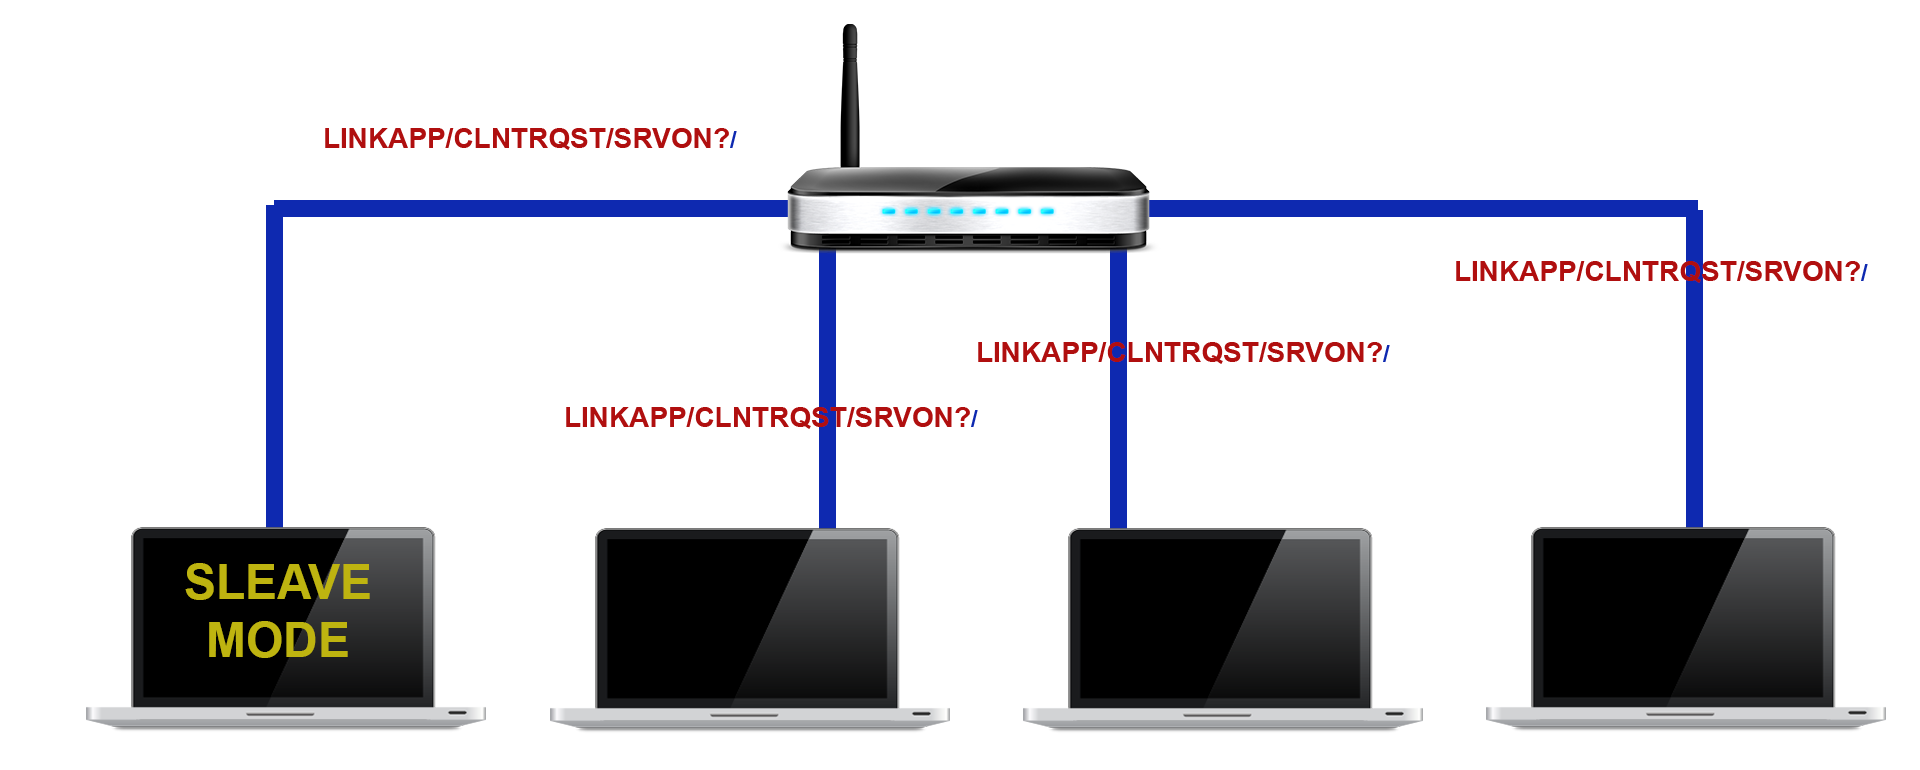
\includegraphics[width=0.77\textwidth]{broadcast.png}
    \caption{Lo sleave invia un messaggio in broadcast per conoscere la rete in cui si trova.}
    \label{fig:awesome_image}
	\centering
    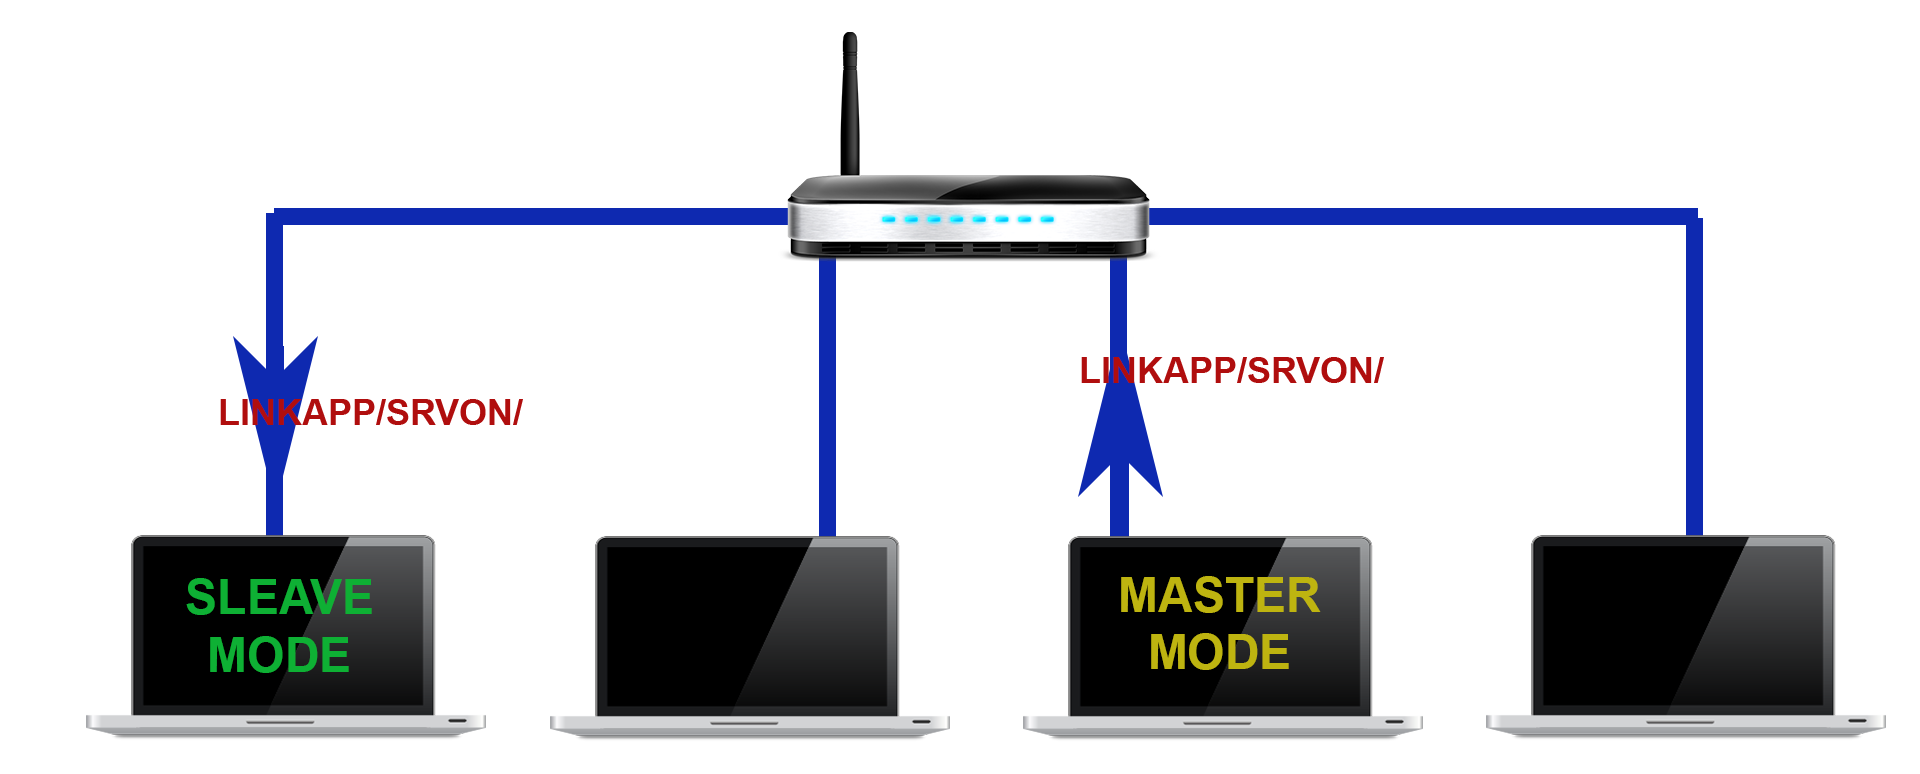
\includegraphics[width=0.77\textwidth]{serveron.png}
    \caption{I master disponibili rispondono alla richiesta dello sleave confermando di essere attivi.}
    \label{fig:awesome_image}
\end{figure}

\subsection{Master}
Per quanto riguarda la modalità master, inizialmente viene aperto un socket UDP il quale si mette in ascolto sulla porta 1235 di eventuali richieste da parte degli sleave. Ricevuta e validata la richesta,il master, dunque, risponde al richiedente con il messaggio di servizio \texttt{LINKAPP/SRVON/<nomemaster>}.
Quindi, dopo aver inviato le proprie informazioni, la piattaforma apre un socket TCP sulla porta 2346 e resta in attesa delle richieste di connessione.
Stabilita la connessione, viene ricevuta la richiesta del file da trasmettere e una, volta validata, viene lasciata la libertà all'utente di accettare o meno lo scambio di file. In caso di esito negativo, il master invia il messaggio  \texttt{LINKAPP/SEND/NOTACCEPTED/} e si occupa della chiusura della connessione mentre, in caso contrario, si procede con la trasmissione dei dati rispondendo con \texttt{LINKAPP/SEND/ACCEPTED/}.
A questo punto viene ricevuta la dimensione del file trasmesso e si continua a ricevere il file finchè non è stato interamente ricevuto, ovvero finchè il numero di byte letti in entrata non corrisponde alla dimensione del file.

\begin{figure}[h]
	\centering
    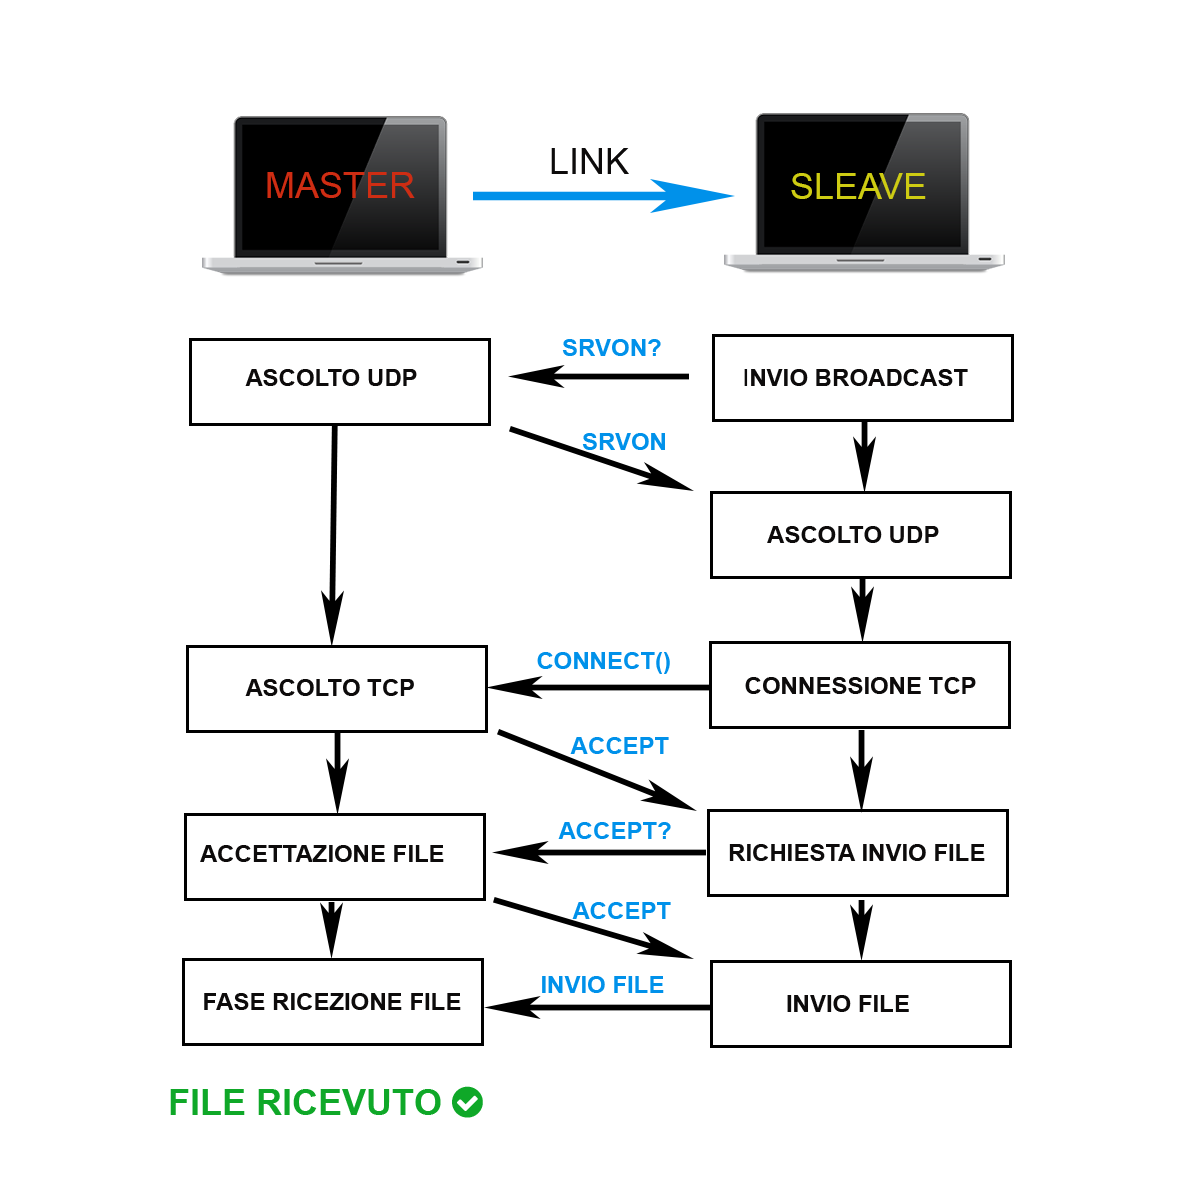
\includegraphics[width=0.77\textwidth]{protocollo.png}
    \caption{Schema del funzionamento della trasmissione dati tra master e sleave.}
    \label{fig:awesome_image}
\end{figure}


\subsection{Compressione dati}\label{Compressione}
Per semplicità e,affinchè fosse possibile comprimere, non solo un singolo file, ma anche una cartella con tutto il suo sottoalbero si è evitato di utilizzare  \texttt{zlib} (solitamente utilizzato in C) ma il meccanismo di  compressione dati è affidato al sistema operativo, in particolare si è scelto di effettuare delle chiamate al sistema per invocare \texttt{tar} applicazione che permette di comprimere file, cartelle e disponibile in tutti i sistemi Unix-like.
Dopo svariate ricerche, si è scoperto che OS X presenta la versione \texttt{bsdtar}, differente dalla tradizionale GNU \texttt{tar}, ma comunque compatibile.

\subsection{Interfaccia utente}
Tra gli obiettivi vi è quello di creare una interfaccia utente piuttosto semplice, pertanto, pur non essendoci una interfaccia grafica si è scelto di utilizzare dei comandi semplici e autoesplicativi attraverso il passaggio di parametri da riga di comando.
Viene pertanto effettuato un parsing dei parametri utilizzando una versione minimizzata di \texttt{Argp} che permette di verificare la correttezza dei parametri passati e, in caso di errore, aiutare l'utente attraverso l' \texttt{---help}.

%----------------------------------------------------------------------------------------
%	CHAPTER 3
%----------------------------------------------------------------------------------------

\chapterimage{develop}
\chapter{Sviluppo e implementazione}

\section{Inizio dello sviluppo}
Trattandosi di uno dei primi grossi progetti personali sviluppati, ed essendo C un linguaggio a me nuovo, la fase di implementazione del codice ha richiesto una parte sostanziale del tempo dedicato al progetto.
Ciò è stato principalmente dovuto a errori di inesperienza nella programmazione C e alla non comprensione della documentazione relativa ai socket di Unix portando più volte alla disperazione.


\section{Implementazione del codice}
In questa sezione vengono documentate le parti più complicate dell'implementazione adottata, in particolar modo come scoprire i master nella rete, il parsing dei parametri da linea di comando, la compressione dei dati e l'utilizzo dei socket per la loro trasmissione.

\subsection{Scoprire i master nella rete}
Una delle funzionalità chiave della piattaforma è sicuramente la possibilità, dopo aver mandato un messaggio broadcast all'intera rete, di trovare i master nelle rete locale pur non conoscendone la struttura. Questa funzionalità è offerta dalla funzione \texttt{srvsInNet()} presente in\texttt{sleave.c}.

Alla funzione viene passato il file descriptor \texttt{udpClntSock} del socket UDP aperto e un array vuoto di \texttt{srv} contenente informazioni sui socket dei master trovati nella rete.
All'interno della funzione viene inizializzato un server fittizio e, successivamente, si imposta il socket in modalità non-blocking, ovvero l'esecuzione del programma non viene interrotta in attesa di dati messaggi in ingresso, proprio per questo viene impostato un tempo massimo per la ricerca.
\begin{lstlisting}[language=C]
int srvsInNet(const int udpClntSock, srv *srvs) {

	//number of server
	int nSrvs = 0;

	struct sockaddr_in currentAddr;
	currentAddr.sin_family = AF_INET;
	currentAddr.sin_port = htons(UDP_SERVER_PORT);
	currentAddr.sin_addr.s_addr = htonl(INADDR_ANY);

	int currentAddrLen = sizeof(currentAddr);

	printf("Waiting for master response...\n");

	//set socket non blocking
	fcntl(udpClntSock, F_SETFL, O_NONBLOCK);
	int err;

	//buffer created
	char buffer[SERVICE_BUFFER_SIZE];

	int excededTime = time(0) + SERVER_SEARCH_TIME;
\end{lstlisting}

A questo punto, finchè il numero di master trovati è minore del numero massimo di quelli rilevabili e non si è superato il tempo massimo di ricerca, si rimane in attesa di messaggi da parte dei server disponibili, viene verificata la validità ed aventualmente si aggiungono tutte le informazioni del master trovato, comprensivo di indirizzo reale, nell'array \texttt{srvs}. Si conclude restituendo il numero di master trovati.

\begin{lstlisting}[language=C]
while ((nSrvs <= MAX_NUMBER_SERVERS ) && (time(0) < excededTime) ) {
	//cleaning buffer
	bzero(buffer, SERVICE_BUFFER_SIZE);

	//checking received message
	recvfrom(udpClntSock, buffer, SERVICE_BUFFER_SIZE, 0, (struct sockaddr *) &currentAddr, &currentAddrLen);
	err = errno;

	//handle error from recvfrom
	if ((err != EAGAIN) && (err != EWOULDBLOCK)) {
      	printf("recv returned unrecoverable error(errno=%d)\n", err);
      	return -1;
      }
	char *strName;
	//checking received message
	if (strncmp(buffer, VALID_SERVER_ON, 14) == 0) {

		//getting server name
		strtok(buffer, "/");
		strtok(NULL, "/");
		strName = strtok(NULL, "/");
		srv currentSrv;
		strcpy(currentSrv.name, strName);
		currentSrv.sockAddr = currentAddr;
		currentSrv.sockAddrLen  = sizeof(currentSrv.sockAddr);

		srvs[nSrvs] = currentSrv;
		nSrvs++;

	}	
}

return nSrvs;

\end{lstlisting}

\subsection{Connessione TCP}
La connessione TCP permette di assicurarci una trasmissione dei dati affidabile e orientata alla connessione (pertanto ordinata). Vediamo quindi come il master apre il socket TCP e si metta in ascolto di eventuali richieste.
Ciò è disponibile in \texttt{master.c} e in particolare nelle funzioni \texttt{masterMode()} e \texttt{openTcpSrv()}.

Inizialmente nella funzione \texttt{masterMode()} viene inizializzata la struttura \texttt{sockaddr\_in} contenente l'indirizzo del socket TCP del master, in particolare gli si assegna la famiglia \texttt{AF\_INET} che permette lo scambio di dati in rete, la porta \texttt{TCP\_SERVER\_PORT} = 2346 e gli si assegna l'intefaccia di loopbak (si imposta in ascolto in tutte le interfacce di rete disponibili).
Successivamente si crea il socket di tipo \texttt{SOCK\_STREAM} effettuando i vari controlli sull'avvenuta creazione:
\begin{lstlisting}[language=C]
//server TCP address
struct sockaddr_in tcpSrvSockAddr;
memset(&tcpSrvSockAddr, 0, sizeof(tcpSrvSockAddr));

tcpSrvSockAddr.sin_family = AF_INET;
tcpSrvSockAddr.sin_port = htons(TCP_SERVER_PORT);
tcpSrvSockAddr.sin_addr.s_addr = htonl(INADDR_ANY);

int tcpSrvSockAddrLen = sizeof(tcpSrvSockAddr);

//client TCP address
struct sockaddr_in tcpClntSockAddr;

int tcpClntSockAddrLen = sizeof(tcpClntSockAddr);


//create TCP server socket
int tcpSrvSock = socket (AF_INET, SOCK_STREAM, 0);

if (tcpSrvSock < 0) {
	perror("\nCannot create TCP server socket: ");
	return -1;
}
\end{lstlisting}

Nella parte successiva, invece il socket viene bindato, ovvero si associa il socket a uno specifico indirizzo assegnato, in questo caso a \texttt{tcpSrvSockAddr}, e vi è una chiamata alla funzione \texttt{openTcpSrv()} passando come parametri il socket creato, il suo indirizzo comprensivo di dimensione, l'indirizzo e la dimensione del socket dello sleave e infine la connessione accettata.

\begin{lstlisting}[language=C]
if (bind(tcpSrvSock, (struct sockaddr *) &tcpSrvSockAddr, tcpClntSockAddrLen) < 0) {
	perror("\nCannot bind TCP server socket: ");
	return -1;
}

//create socket for connection 
int connectionSock;
int tcpSrvIsOpen = openTcpSrv(tcpSrvSock, (struct sockaddr_in *)&tcpSrvSockAddr,
  tcpSrvSockAddrLen, (struct sockaddr_in *)&tcpClntSockAddr, tcpClntSockAddrLen,
  &connectionSock);

\end{lstlisting}

Nella funzione \texttt{openTcpSrv()} pertanto si pone il socket in ascolto imponendogli una backlog di 5, ovvero limitando il numero di connessioni in sospeso nella coda del socket. Successivamente, le richieste di connessione vengono accettate mediante la funzione \texttt{accept()} e vengono salvate in \texttt{connectionSock} permettendo dunque di iniziare la trasmissione dei dati.
\begin{lstlisting}[language=C]
int openTcpSrv(const int tcpSrvSock, struct sockaddr_in *tcpSrvSockAddr, const int tcpSrvSockAddrLen, struct sockaddr_in *tcpClntSockAddr, int tcpClntSockAddrLen, int *connectionSock) {

	printf("\nStarting TCP server...\n");
	fflush(stdout);
	//start listening with queue size of 5
	if(listen(tcpSrvSock, 5) < 0) {
		printf("Error starting listening\n");
		// exit(1);
	}

	//search for a connection request
	int request;
	while (1) {

		printf("ConnectionSock: %d\n", connectionSock);
		//accept connection with sleave
		request = accept(tcpSrvSock, (struct sockaddr *) &tcpClntSockAddr, &tcpClntSockAddrLen);

		printf("ConnectionSock after accept: %d\n", request);

		*connectionSock = request;
		
		
		if(connectionSock < 0) {
			perror("Connection with sleave not accepted: ");
			return -1;
		}

		return 0;
	}
	
}
\end{lstlisting}

\subsection{Ricezione del file}
Sicuramente la ricezione del file rappresenta il cuore della piattaforma realizzata in quanto permette di raggiungere l'obiettivo primario, ovvero la trasmissione dei dati da un host a un altro. E' pertanto qui riportata la documentazione relativa alla funzione \texttt{receiveFile()} presente in \texttt{master.c}.

Dopo che l'utente ha accettato il file il master invia un messaggio allo sleave comunicandogli di poter iniziare la trasmissione; viene ricevuta la dimensione del file da ricevere e successivamente, si apre, con lo stesso nome del file in ricezione, un file in modalità di scrittura.


\begin{lstlisting}[language=C]
int receiveFile (const int *connectionSock, const char *fileToReceive) {

char buffer[DATA_BUFFER_SIZE];

send(connectionSock, SEND_ACCEPTED, sizeof(SEND_ACCEPTED), 0);
printf("Server response:%s\n", SEND_ACCEPTED);

//creating service buffer for receiving file size
char serviceBuffer[SERVICE_BUFFER_SIZE];
memset(&serviceBuffer, 0, sizeof(serviceBuffer));

//receiving buffer size
recv(connectionSock, serviceBuffer, sizeof(serviceBuffer),  0);
printf("buffer: %s\n", serviceBuffer);

//transform buffer into a int
int size = atoi(serviceBuffer);
printf("File size to receive: %d\n", size);

// opening file
FILE *fpOutput;
fpOutput = fopen(fileToReceive, "w");

if(fpOutput == NULL) {
	printf("NONO\n");
}

\end{lstlisting}

Dunque si inizia a ricevere il file e si continua a leggere nel socket finchè i byte letti non corrispondono alla effettiva dimensione del file.

\begin{lstlisting}[language=C]
//byte read
int offset = 0;
int n;

// receiving message
while( n = read(connectionSock, buffer, sizeof(buffer)) > 0 && offset < size) {
	fwrite(buffer, DATA_BUFFER_SIZE, 1, fpOutput);
	// printf("%s", buffer);
	offset = offset + n;
}

return 0;

\end{lstlisting}

\subsection{Argp e il parsing dei comandi}
Grazie all'utilizzo di una piccola libreria basata su Argp di GNU  è stato possibile effettuare, in modo elegante e sicuro, il parsing dei parametri da linea di comando, in particolare, esso, infatti, ci permette di costringere l'utente all'utilizzo dei comandi designati. Analizziamo nei dettagli la sua implementazione presente in \texttt{link.c}.\\
\texttt{Argp} ci fornisce la struttura \texttt{arpg\_option} con la quale andiamo a specificare ogni parametro utilizzato
\begin{lstlisting}[language=C]
struct argp_option {
    char *name;
    char  key;
    char *arg;
    int   flags;
    char *doc;
    int   group;    
};
\end{lstlisting}
In cui:
\medskip
\begin{description}
	\item [\texttt{name}] rappresenta il nome dell'opzione;
	\item [\texttt{key}] è la chiave che viene passata al parser per riconoscere l'opzione;
	\item [\texttt{arg}] è l'argomento dell'opzione (se ce ne sono);
	\item [\texttt{flags}] rappresenta i flag dell'opzione;
	\item [\texttt{doc}] è una stringa di documentazione per l'opzione.
\end{description}
\medskip

\noindent E inoltre ci mette a diposizione la struttura \texttt{argp\_state} dove vengono salvate le informazioni relative allo stato del parsing corrente.

\noindent Pertanto andiamo a definire le opzioni che accettiamo da linea di comando, ovvero:
\begin{lstlisting}[language=C]
	static struct argp_option options[] = {
  {"verbose", 'v', 0, 0, "Produce verbose output" },
  {"listen", 'l', 0, 0, "Start listening" },
  {"send", 's', "<FILENAME>", 0, "Send file"},
  {"setname", 'n', "<NEWNAME>", 0, "Set user name" },
  {"getname", 'g', 0, 0, "Get user name"},
  { 0 }
};
\end{lstlisting}
Dove abbiamo definito:
\medskip
\begin{description}
	\item [\texttt{verbose}] stampa i vari passaggi dell'operazione eseguita (attualmente di default);
	\item [\texttt{listen}] avvia la master mode;
	\item [\texttt{send}]  seguito dall'argomento \texttt{<filename>} attiva la sleave mode e invia il file avente nome 					\texttt{filename};
	\item [\texttt{setname}] seguito dall'argomento \texttt{<newname>} imposta il nuovo nome utente \texttt{newname};
	\item [\texttt{getname}] stampa sullo schermo il proprio nome utente.
\end{description}
\medskip

Successivamente ci occupiamo di definire la struttura argomenti che verrà passata ad \texttt{Argp} e viene utilizzata dal main per comunicare con la funzione \texttt{argp\_opt} che definiremo nel prossimo passaggio:
\begin{lstlisting}[language=C]
struct arguments {
  char *args[2];                /* arg1 & arg2 */
  int listen, verbose, getName;
  char *sendFile;
  char *newName;
};
\end{lstlisting}

Quindi abbiamo la funzione che, un parametro alla volta, verificare la correttezza di quanto passato e, in caso di riconoscimento setta le variabili corrispondenti, altrimenti fissa lo stato su \texttt{ARGP\_ERR\_UNKNOWN}.
In caso, invece in cui il numero di parametri passati sia superiore rispetto a quelli dovuti verrà fissato lo stato \texttt{ARGP\_KEY\_ARG} mentre terminato il parsing \texttt{ARGP\_KEY\_END}

\begin{lstlisting}[language=C]
static error_t parse_opt (int key, char *arg, struct argp_state *state) {
  /* Get the input argument from argp_parse, which we
     know is a pointer to our arguments structure. */
  	struct arguments *arguments = state->input;

  	switch (key) {
    	case 'l':
      		arguments->listen = 1;
      		break;
    	case 'v':
      		arguments->verbose = 1;
      		break;
    	case 'g':
      		arguments->getName = 1;
      		break;		
    	case 'n':
      		arguments->newName = arg;
      		break;		
    	case 's':
      		arguments->sendFile = arg;
      		break;
      		
    	case ARGP_KEY_ARG:
      		if (state->maxlen >= 2) {
        		argp_usage (state);
        	}

      		arguments->args[state->maxlen] = arg;
      		break;
    	case ARGP_KEY_END:
      		if (state->maxlen < 2) {
     			argp_usage (state);
     		}
      		break;
    	default:
      		return ARGP_ERR_UNKNOWN;
    }

  return 0;
  
}

\end{lstlisting}

Andiamo dunque a costruire la struttura da passare ad argp per il parsing
\begin{lstlisting}[language=C]
static struct argp argp = { options, parse_opt, args_doc, doc };
\end{lstlisting}
\noindent In cui \texttt{options}, \texttt{parse\_opt} sono stati già definiti mentre \texttt{args\_doc} e \texttt{doc} sono delle stringhe contenenti rispettivamente informazioni sui parametri da passare e sull'applicazione.

\noindent Nella funzione \texttt{main()}, pertanto, dopo aver inizializzato la struttura \texttt{arguments}, effettuiamo la chiamata al parser di Argp

\begin{lstlisting}[language=C]
argp_parse (&argp, argc, argv, 0, 0, &arguments);
\end{lstlisting}


\subsection{Chiamate di sistema}
Un'altra parte interessante del codice sono sicuramente le chiamate a sistema che legano questa piattaforma ai sistemi operativi Unix-like.
In particolare sono state effettuate due principali chiamate:
\medskip
\begin{description}
	\item[Compressione]: per effettuare la compressione del file/cartella da inviare è stata effettuata una chiama al sistema attraverso la funzione 			\texttt{system()} presente nella \texttt{stdio.h} la quale ha permesso di chiedere al sistema operativo dell'host di eseguire il comando 				desiderato. Avendo scelto di utilizzare \texttt{tar}, il comando \texttt{tarCommand} non è altro che la stringa "tar -zcf <filename>.tar.gz 			<filename>"
\end{description}

\begin{lstlisting}[language=C]
	system(tarCommand);
\end{lstlisting}

\begin{description}
		
	\item[Verifica esistenza file]: per verificare l'esistenza del file/cartella sono stati utilizzati i comandi della bash \texttt{[ -f <nomefile> 			]}/\texttt{[ -d <nomecartella> ]} ma, affinchè il risultato di questa chiamata fosse poi computabile è stato necessario aprire una pipe con la 			shell nella funzione \texttt{exists()}		
\end{description}
\medskip
Inizialmente, nella funzione \texttt{exists()}, è stata modificata la chiamata al sistema in base al tipo di file da inviare, infatti, nel caso in cui sia necessario effettivamente un file la chiamata al sistema dovrà essere \texttt{[ -f <nomefile> ]} mentre, nel caso in cui si debba inviare una cartella, dovrà essere \texttt{[ -d <nomefile> ]}.
Pertanto il comando di sistema che verifica l'esistenza del file/cartella viene costruito in modo tale che la shell restituisca il carattere '1' in caso di esito positivo, '0 altrimenti'.
\begin{lstlisting}[language=C]
char exists(const char *fileName, char c) {

	if (c != 'f' && c != 'd') {
		printf("Argument not valid");
		return 0;
	}

	//construction of system call for verifying if file exists
	char existsCommand[EXISTS_COMMAND_SIZE];
	memset(&existsCommand, 0, sizeof(char) * EXISTS_COMMAND_SIZE);

	if (c == 'f') {
		strcpy(existsCommand, "[ -f ");
	} else {
		strcpy(existsCommand, "[ -d ");
	}

	strcat(existsCommand, fileName);
	strcat(existsCommand, " ] && echo 1 || echo 0");
\end{lstlisting}

Quindi, per poter utilizzare il risultato di tale chiama, vi è la necessità di aprire una pipe con la shell, effettuare un forking e reindirizzare l'output su un I/O stream attraverso la funzione popen.

\begin{lstlisting}[language=C]
	// open pipe with unix shell
	FILE *fp;
	fp = popen(existsCommand, "r");

	if (fp == NULL) {
    	printf("Failed to run command\n" );
    	exit(1);
  	}

  	char result = fgetc(fp);
\end{lstlisting}

%----------------------------------------------------------------------------------------
%	CHAPTER 4
%----------------------------------------------------------------------------------------

\chapterimage{bridgetest} % Chapter heading image

\chapter{Valutazione e collaudo}

\section{Testing sul campo}
La fase di sviluppo dell'applicazione è stata un susseguirsi di implementazione e testing delle nuove funzionalità. In particolare, sfruttando il fatto che master e sleave lavorano con socket bindati a porte differenti, è stato possibile testare la piattaforma semplicemente utilizzando in parallelo due shell di comando in cui da una parte si attiva la masterMode, mentre dall'altra la sleaveMode.
Riportiamo di seguito il risultato dei test principali eseguiti, comprensivi di messaggi utili per la comprensione di quanto l'applicazione sta realmente facendo, a sinistra avremo il master, mentre a destra abbiamo lo sleave:

\begin{Parallel}{0.5\textwidth}{0.5\textwidth}
\ParallelLText{
\begin{lstlisting}[language=Bash]
MacBook-Pro-di-Davide-3:master davidetalon$ link --listen

Waiting for sleave...
\end{lstlisting}
}
\ParallelRText{
\begin{lstlisting}[language=Bash]
MacBook-Pro-di-Davide-3:sleave davidetalon$ link --send canzone.mp3
Broadcast sent: LINKAPP/CLNTRQT/SRVON?
Waiting for master response...
1 masters found

0. Tallo
Scegliere un master valido:
\end{lstlisting}
}
\ParallelPar
\end{Parallel}

Mentre dal lato master viene aperto il socket Udp in ascolto per eventuali richieste, dal lato sleave vengono inviati i pacchetti 				broadcast e si stabiliscono i server attivi all'interno della rete, dando la possibilità all'utente di scegliere il destinatario.

\begin{Parallel}{0.5\textwidth}{0.5\textwidth}
\ParallelLText{
\begin{lstlisting}[language=Bash]
MacBook-Pro-di-Davide-3:master davidetalon$ link --listen

Waiting for sleave...UDP request: LINKAPP/CLNTRQT/SRVON?
Server response: LINKAPP/SRVON/Tallo
Starting TCP server...
ConnectionSock: 1514626604
\end{lstlisting}
}
\ParallelRText{
\begin{lstlisting}[language=Bash]
MacBook-Pro-di-Davide-3:sleave davidetalon$ link --send canzone.mp3
Broadcast sent: LINKAPP/CLNTRQT/SRVON?
Waiting for master response...
1 masters found

0. Tallo
Scegliere un master valido: 0
Connetcting to Tallo...
Connection enstabilished.
tarCommand command: tar -zcf canzone.mp3.tar.gz canzone.mp3
Header sent: LINKAPP/SLVNAME/Tallo/FNAME/canzone.mp3.tar.gz/
Header size: 336
\end{lstlisting}
}
\ParallelPar
\end{Parallel}

Ricevuta la richiesta da parte dello sleave il master attiva il socket TCP e resta in attesa di eventuali connessioni, dall'altra parte lo sleave si connette al master ed invia l'header contenente il proprio username e il nome del file da inviare.

\begin{Parallel}{0.5\textwidth}{0.5\textwidth}
\ParallelLText{
\begin{lstlisting}[language=Bash]
MacBook-Pro-di-Davide-3:master davidetalon$ link --listen

Waiting for sleave...UDP request: LINKAPP/CLNTRQT/SRVON?
Server response: LINKAPP/SRVON/Tallo
Starting TCP server...
ConnectionSock: 1514626604
ConnectionSock after accept: 6
Connection enstabilished
ConnectionSock: 6
Header: LINKAPP/SLVNAME/Tallo/FNAME/canzone.mp3.tar.gz/
Accept file canzone.mp3.tar.gz from Tallo? (Y/N)
\end{lstlisting}
}
\ParallelRText{
\begin{lstlisting}[language=Bash]
MacBook-Pro-di-Davide-3:sleave davidetalon$ link --send canzone.mp3
Broadcast sent: LINKAPP/CLNTRQT/SRVON?
Waiting for master response...
1 masters found

0. Tallo
Scegliere un master valido: 0
Connetcting to Tallo...
Connection enstabilished.
tarCommand command: tar -zcf canzone.mp3.tar.gz canzone.mp3
Header sent: LINKAPP/SLVNAME/Tallo/FNAME/canzone.mp3.tar.gz/
Header size: 336
Server response: LINKAPP/SEND/ACCEPTED/
Opening file canzone.mp3.tar.gz ...
size: 7210143
Remove command: rm -r canzone.mp3.tar.gz
File succefully sent.
\end{lstlisting}
}
\ParallelPar
\end{Parallel}

Grazie all'header precedentemente trasmesso il master ha le informazioni necessarie per chiedere all'utente se desidera accettare il file in ingresso, nella master mode, invece, una volta che il file è stato accettato esso viene inviato con successo.

\noindent Infine notiamo come il file sia realmente giunto a destinazione e sia valido, infatti è possibile estrarlo.

\begin{lstlisting}[language=Bash]
MacBook-Pro-di-Davide-3:master davidetalon$ link --listen

Waiting for sleave...UDP request: LINKAPP/CLNTRQT/SRVON?
Server response: LINKAPP/SRVON/Tallo
Starting TCP server...
ConnectionSock: 1514626604
ConnectionSock after accept: 6
Connection enstabilished
ConnectionSock: 6
Header: LINKAPP/SLVNAME/Tallo/FNAME/canzone.mp3.tar.gz/
Accept file canzone.mp3.tar.gz from Tallo? (Y/N) y

Receiving file canzone.mp3.tar.gz from Tallo...
Server response:LINKAPP/SEND/ACCEPTED/
buffer: 7210143
File size to receive: 7210143
MacBook-Pro-di-Davide-3:master davidetalon$ ls
canzone.mp3.tar.gz
MacBook-Pro-di-Davide-3:master davidetalon$ tar -xzf canzone.mp3.tar.gz
MacBook-Pro-di-Davide-3:master davidetalon$ ls
canzone.mp3		canzone.mp3.tar.gz
\end{lstlisting}


\section{Valutazione e bug riscontrati}
Osservando l'output dei terminali relativi allo sleave e al master è possibile confermare la correttezza dei risultati e verificare il soddisfamento delle specifiche che avevamo prefissato come obiettivo. Tuttavia sono stati riscontrati alcuni bug che compaioni in determinate condizioni:
\begin{description}
	\item[Unrecoverable error]: alcune volte capita che, nel socket UDP dello sleave, la \texttt{recvfrom()} dia "Unrecoverable error" errno = 9 Bad 		file number (motivo non ancora identificato);
	\item[File name invalid encoding]: nella trasmissione dati da un sistema operativo OS X ad Ubuntu il nome del file assume una codifica non 			valida, tale problema è dovuto alla differente codifica dei caratteri nei due sistemi operativi;
	\item[Address already in use]: lo sleave tentando di connettersi al server (TCP) utilizza un indirizza già in uso 
\end{description}




%----------------------------------------------------------------------------------------
%	CHAPTER 5
%----------------------------------------------------------------------------------------

\chapterimage{windowsout} % Chapter heading image

\chapter{Conclusioni e lavoro futuro}

\section{Lavoro futuro}
L'applicazione si trova tuttora a uno stato embrionale, infatti, possono essere fatte numerose interessanti modifiche che permettono di estenderne le funzionalità e di allargarne l'utenza. 
Alcune interessanti idee sono sicuramente:
\begin{description}
	\item[Correzione bugs]: risolvere i problemi attualmente riscontrati
	\item[Porting su Windows]: uno dei prossimi obiettivi sarà sicuramente quello di rendere disponibile l'applicazione anche per utenti Windows 			permettendo dunque di raggiungere la gran parte del mercato. Ciò comporta un carico di lavoro abbastanza elevato,in quanto, non solo dobbiamo 			adattare i socket a Winsock ma dobbiamo adattare le varie chiamate del sistema, in particolare:
			\begin{itemize}
				\item la verifica dell'esistenza o meno del file da inviare
				\item la compressione dei dati da inviare, infatti Windows non fornisce una libreria  per la compressione di dati,contrariamente a 					quanto avviene nei sistemi Unix-like
			\end{itemize}
	\item[Introduzione crittografia end-to-end]: è possibile introdurre una crittografia E2EE per rendere la trasmissione dei file sicura e 				impenetrabile contro i malintenzionati
	\item[Più formati di compressione]: è inoltre doveroso implementare più sistemi di compressione per lasciare all'utente la possibilità di 				scegliere il formato di compressione desiderato
\end{description}

Ci si augura di poter continuare a lavorare sul progetto in quanto le soddisfazioni e le conoscenze tecniche aumentano in maniera esponenziale.


\section{Conclusioni}
Posso ritenermi soddisfatto di quanto realizzato in questo progetto in quanto, oltre ad avermi permesso di risolvere un problema che affrontavo quotidianamente, mi ha dato l'occasione di accrescere le mie conoscenze sulla programmazione e in particolare sui principi fondamentali delle trasmissioni di dati.
Durante la fase di progettazione e di implementazione ho affrontato problematiche mai incontrate  prima (un po' per le novità del linguaggio un po' per generale inesperienza) come ad esempio il parsing efficiente dei comandi da riga di comando o la necessità, in una trasmissione dati, di tener traccia di quanto effettivamente inviato e ricevuto.

Inoltre confrontarmi con la documentazione scritta da altri programmatori mi ha permesso di comprendere quanto sia importante, non solo commentare il codice, ma anche redarre una documentazione chiara e completa.
Infine per la prima volta mi sono imbattuto in un potente strumento come CMake utile per lo sviluppo di codice da distribuire.

Ringrazio in particolar modo \url http://stackoverflow.com/ e tutta la sua community per tutti i preziosi consigli suggeritimi.

\vfill
\textit{Davide Talon}
\end{document}